\section{Stripe}
\label{sec:stripe}
Stripe is the best way to accept payments online. Stripe aims to expand internet commerce by making it easy to process transactions and manage an online business.
\newline
Stripe is 365 people and headquartered in an old trunk factory in the Mission district of San Francisco. The company has received around \$300 million in funding to date; investors include Sequoia Capital, Visa, American Express, Peter Thiel, and Elon Musk. Stripe enables you to accept payments in minutes. Collect your customers’ payment information easily and securely on web or mobile, and create charges server-side. Stripe supports 100+ currencies out of the box. In addition to credit and debit cards, Apple Pay, Android Pay, you can also easily support Bitcoin, Alipay, or Amex Express Checkout.
\subsection{How it work}
Even Stripe, as Braintree, provides a default widget that you can use to integrate payments.
\begin{figure}[htb]
  \centering
  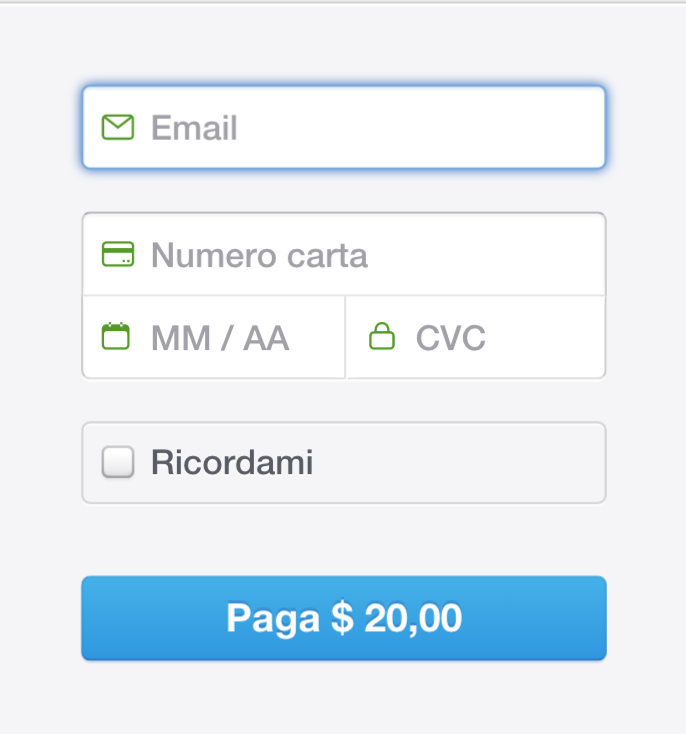
\includegraphics[width=0.5\linewidth]{images/chapter4/stripe-drop.png}\hfill
  \caption[Default stripe payment widget]{Default stripe payment widget}
\label{fig:stripe_default_ui}
\end{figure}
To get this widget, just enter the following code in its page:
\begin{lstlisting}[language=html]
<form action="" method="POST">
  <script
    src="https://checkout.stripe.com/checkout.js" class="stripe-button"
    data-key="pk_test_6pRNASCoBOKtIshFeQd4XMUh"
    data-amount="2000"
    data-name="Demo Site"
    data-description="2 widgets ($20.00)"
    data-image="/128x128.png"
    data-locale="auto">
  </script>
</form>
\end{lstlisting}
The most important thing to notice is the data-key attribute added to the script tag. This key identifies your account when communicating with Stripe.
\newline
Stripe also offers the ability to customize the payment form. This and other details can be discussed in Chapter 5.